\documentclass[11pt, a4paper]{report}

\usepackage{geometry}
\usepackage[utf8]{inputenc}
\usepackage[english]{babel}
\usepackage[T1]{fontenc}

\usepackage{graphicx} % Required for including pictures
\usepackage{float} % Allows putting an [H] in \begin{figure} to specify the exact location of the figure
\usepackage{pdfpages}
\usepackage{booktabs}
\usepackage{tabularx}
\restylefloat{table}
\usepackage{listings}
\usepackage{dirtytalk}

\usepackage{tikz}
\usepackage{forest}
\usepackage{caption}
\usepackage{subcaption}
\usepackage{wrapfig} % Allows in-line images such as the example fish picture

\usepackage{lmodern} % load a font with all the characters

\linespread{1.2} % Line spacing

%\setlength\parindent{0pt} % Uncomment to remove all indentation from paragraphs

\graphicspath{{Pictures/}} % Specifies the directory where pictures are stored

\renewcommand{\baselinestretch}{1.3}
\headsep = 10.mm
%%%% CHOOSE MARGINS %%%%

\geometry{hmargin=2.5cm,top=3cm,bottom=2.3cm}
%%%% COMMANDS %%%%
%%%%%%%%%%%%%%%%%%%%%%%%%%%%%%%%%%%%% CHANGE HERE %%%%
\renewcommand\title{UCLCampus: a moblie application for UCL students}
\newcommand\nameone{Arnold \textsc{Moyaux}}
\newcommand\nametwo{Baptiste \textsc{Lacasse}}
\newcommand\options{}
\newcommand\supervisor{Yves \textsc{Deville}}
\newcommand\readerone{Kim \textsc{Mens}}
\newcommand\readertwo{Hildeberto \textsc{Mendonça}}
\newcommand\readerthree{Mathieu \textsc{Zen}}
\newcommand\readerfour{Jorge \textsc{Perez Medina}}
\newcommand\years{2015-2016}
%%%% BEGIN %%%%
\begin{document}

%%%% COVER %%%%
\thispagestyle{empty}
\noindent\begin{minipage}{.25\textwidth}
\noindent
\includegraphics[width=3.6cm]{Images/ucl.jpg}
\end{minipage}
\begin{minipage}{.5\textwidth}
\begin{center}
UNIVERSITE CATHOLIQUE DE LOUVAIN
\\~\\~
ECOLE POLYTECHNIQUE DE LOUVAIN
\\~\\~\\~\\~\\~
\end{center}
\end{minipage}
\begin{minipage}{.25\textwidth}
\hfill
\includegraphics[width=3.6cm]{Images/epl.jpg}
\\~\\~\\~\\~
\end{minipage}
\vspace{4.5cm}
\begin{center}
\bfseries{\scshape{\Huge{\title}}}
\end{center}
\vspace{4.5cm}
\begin{minipage}{.5\textwidth}
\begin{tabular}{ll}
Supervisor: & \supervisor
\\ Readers: & \readerone 
\\          & \readertwo 
\\          & \readerthree
\\          & \readerfour
\end{tabular} 
\\~\\~
\end{minipage}
\begin{minipage}{.5\textwidth}
\begin{tabular}{l}
Thesis submitted for the Master's degree
\\ in computer science and engineering
\\ options: \
\\ by : \nameone
\\ 	   \nametwo
\end{tabular}
\end{minipage}
\vfill
\begin{center}
Louvain-la-Neuve
\\ Academic year \years
\end{center}
%%%% END COVER %%%%
%----------------------------------------------------------------------------------------
%	TABLE OF CONTENTS
%----------------------------------------------------------------------------------------

\tableofcontents % Include a table of contents

\newpage % Begins the essay on a new page instead of on the same page as the table of contents 


\chapter{Introduction} % Major section

Brief introduction of the project, the goals and the contents of the rest of the thesis.


\chapter{Background}

In this section, we will look at the different existing technologies relating to the different aspects of our project and will explain the choices we made. // TODO

\section{Cross-platform mobile development tools}

In each of these sections, we will detail the different approaches one could choose to develop a cross-platform moblie applications. We will also present several frameworks using these approaches. We will then compare them and choose one of those approaches for the rest of the project. //TODO
\subsection{The native approach}

The first approach we considered for our project was what we call a native approach. The native approach consists in using the native technology and language for each platform, for instance Java for Android and Objective-C for iOS.  

\begin{table}[H]
\begin{tabularx}{\linewidth}{>{\parskip1ex}X@{\kern4\tabcolsep}>{\parskip1ex}X}
\toprule
\hfil\bfseries Pros
&
\hfil\bfseries Cons
\\\cmidrule(r{3\tabcolsep}){1-1}\cmidrule(l{-\tabcolsep}){2-2}

Best achievable performance\par
Always up-to-date with the latest API\par
Can use any platform\par

&

Low maintainability\par
Harder to find contributors fluent in all technologies\par
Can lead to different versions of the application\par


\\\bottomrule
\end{tabularx}
\caption{Pros and cons of the native approach}
\end{table}

\subsection{The web approach}
A second approach we considered was the web approach. This approach consists in using HTML5 to develop an application that will be usable on any platform.


\begin{table}[H]
\begin{tabularx}{\linewidth}{>{\parskip1ex}X@{\kern4\tabcolsep}>{\parskip1ex}X}
\toprule
\hfil\bfseries Pros
&
\hfil\bfseries Cons
\\\cmidrule(r{3\tabcolsep}){1-1}\cmidrule(l{-\tabcolsep}){2-2}

Can be used on any mobile platform\par
Easy to find contributors fluent in HTML5\par
Easy to maintain\par

&

Doesn't have access to native platform features\par
Harder to implement local storage/security (//TODO NEED BETTER SOURCE)\par
Not as performant as native\par



\\\bottomrule
\end{tabularx}
\caption{Pros and cons of the web approach}
\end{table}
\subsection{The hybrid approach}

The last approach to develop a mobile application is called the hybrid approach. An hybrid app is mostly built using HTML5 and JavaScript and is then wrapped inside a thin native container, giving it access to native features.

\begin{table}[H]
\begin{tabularx}{\linewidth}{>{\parskip1ex}X@{\kern4\tabcolsep}>{\parskip1ex}X}
\toprule
\hfil\bfseries Pros
&
\hfil\bfseries Cons
\\\cmidrule(r{3\tabcolsep}){1-1}\cmidrule(l{-\tabcolsep}){2-2}

Can be used on any mobile platform\par
Easy to find contributors fluent in HTML5 and JavaScript\par
Easy to maintain\par

&

Not as performant as native\par



\\\bottomrule
\end{tabularx}
\caption{Pros and cons of the hybrid approach}
\end{table}

\subsection{Our choice}

\section{Open-source project and code sharing}

In this section, we will explain the choices we made concerning the code sharing platforms we used as well as the licenses we used to protect our work.

\section{Project Management Methodologies}

Here we detail the choices we made as to how we were going to manage de different parts of the project.

\chapter{Functionalities of UCLCampus}

In this part, we will show how we defined the relevant functionalities of our application as well as the user interface.

\section{Choice of functionalities and sections}

//TODO ajouter les trucs qu'on a pas intégré au final (mail, aide, ...)

In order to define what kind of functionalities we wanted to be part of our application, we needed to know what the students needed. The first step was to define a number of user stories that we would then translate into functionalities.\\ 
We split our user stories into several categories:

\begin{itemize}

\item Studies: anything directly related to a user's studies, for instance his classes, the lecture halls or the libraries.
\item Campus: anything related to student life in the campus but not related to the user's studies. For instance "Kot à Projets" or "Cercles".
\item City: anything related to the city the user is in but not related to the university. For instance a cinema or restaurants.
\item Tools: the tools offered by the application that might relate to several other categories. For example the map.
\item Settings: the settings of the application. For example the language or the currently selected campus.

\end{itemize}

We also define two types of users:

\begin{itemize}

\item Students: students can access all the functionalities of the application using their UCL login information. Indeed, some functionalities are student specific. For instance, it wouldn't make sense for a person who isn't a student to try to access his or her schedule.

\item Users: users are people who aren't students but might still be interested in some functionalities the application has to offer. 

\end{itemize}

In our user stories, any story starting by 'as a student' cannot be used by users while any story starting by 'as a user' can be used by both users and students.\\

We will now give a list of the different user stories we thought of for each of our categories.

\subsubsection{Studies}

\begin{itemize}

\item Schedule
\begin{itemize}
\item As a student, I can access my schedule in order to know when my courses are given.
\item As a student, I want to know where a course is given.
\item As a student, I want to know the name of a teacher giving a certain course of my schedule.
\item As a student, I can export my schedule to my phone's agenda so that I don't need Internet access to see it.
\end{itemize}

\item Libraries
\begin{itemize}
\item As a user, I can see whether a library is open or closed.
\item As a user, I can display the address of any library.
\item As a user, I can have a GPS guide to access libraries from my location.
\end{itemize}

\item Lecture halls
\begin{itemize}
\item As a user, I can check the address of any lecture hall.
\item As a user, I can have a GPS guide to access lecture halls from my location.
\end{itemize}

\item Websites
\begin{itemize}
\item As a user, I can quickly access the moodle website through the application.
\item As a user, I can quickly access the UCL website through the application.
\end{itemize}

\end{itemize}

\subsubsection{Campus}

\begin{itemize}

\item{Events}
\begin{itemize} 
\item As a user, I can see a list of events taking place in my campus.
\item As a user, I can sort the events by category.
\end{itemize}

\item{Kots à Projet}
\begin{itemize}
\item As a user, I can check Kots à Projet to know their address and projects.
\item As a user, I can have a GPS guide to access Kots à Projet from my location.
\end{itemize}

\item{Cercles}
\begin{itemize}
\item As a user, I can check "Cercles" to know their address.
\item As a user, I can have a GPS guide to access "Cercles" from my location.
\end{itemize}

\item{Restaurants Universitaires}
\begin{itemize}
\item As a user, I can see the different "Restaurants Universitaires" in my campus.
\item As a user, I can check the menu of the "Restaurants Universitaires".
\item As a user, I can have a GPS guide to access "Restaurant Universitaires" from my location.
\end{itemize}

\item{Sports}
\begin{itemize}
\item As a user, I can see a list of sports organized in my campus.
\item As a user, I can sort the sports by day or by sport.
\end{itemize}

\end{itemize}

\subsubsection{City}

\begin{itemize}

\item Tourism
\begin{itemize} 
\item As a user, I can see the address of the city's information center.
\item As a user, I can see a list of the museums of the city I'm in.
\item As a user, I can see whether a museum is opened or closed.
\end{itemize}

\item Activities
\begin{itemize} 
\item As a user, I can see the address of the city's cinema in order to access it with the help of a GPS guide.
\item As a user, I can see several activities I can do in the city I'm in.

\end{itemize}

\item Restaurants and bars
\begin{itemize} 
\item As a user, I can see a list of the restaurants of the city I'm in.
\item As a user, I can see a list of the bars of the city I'm in.
\end{itemize}

\end{itemize}

\subsubsection{Tools}

\begin{itemize}
\item As a user, I can access a map of the city I'm in in order to check points of interests.
\item As a user, I can receive help from a GPS guide in order to access a location of my choice on the map.
\end{itemize}

\subsubsection{Settings}

\begin{itemize}
\item As a user, I can change the application's language to French, English or Dutch.
\item As a user, I can select my campus.
\end{itemize}

\section{User interface}

Once we determined the different features we wanted in our application, we needed to organize them in a way that makes sense for users. In order to do so, we made sketches of what the application might look like using InVision. InVision is a website that lets people design and style mobile applications prototypes. It allows us to get an idea of what the finished product might look like without having to dive into any code. The sketches we made are available in the annex.\\

In these sketches, we can see that we decided to have one menu per category we defined in the previous section. Each menu has an associated color, allowing the user to always have visual clues to help them know where they are.\\

Once the sketches were done, we shared the link to our prototype to over 1000 students, mostly student in their first year, as they represent the future users of this application. They were able to browse through the application using the buttons, as if it were already working, and leave comments and feedback wherever they wanted to.\\

While we didn't receive as much feedback as we would have hoped, the one we received was constructive and helpful. Most people were satisfied with our 3 first categories, Studies, Campus and City. The fourth category, however, was more criticized. Here are some comments we received concerning the Tools category.\\

\say{[...]\\ 
Quelques remarques:
\begin{itemize}
\item L'icône "Outils" du menu principal pourrait être renommer par soucis de clarté, on s'attend à tomber sur les "outils" ou paramètres de l'application et non pas du campus/ de la ville.
\item Je ne vois pas trop l’intérêt de l'onglet mail étant donné que la plupart des étudiants possédant un smartphone ont déjà leur boite mail étudiant connectée. 
\item L'onglet "Aide" est un peu caché et on ne s'attend pas à trouver ces infos là quand on clique, le lien parking devrait plutôt figurer dans le menu "ville" par exemple. (le renommer "infos utiles", ou qqch de plus parlant que "aide" éventuellement).
\end{itemize}
[...]}\\\\
\say{[...] \\
2. la partie "mails" est sans intérêt puisqu'on est sur un smartphone où la messagerie est probablement déjà configurée.\\
3. le menu "Aide" pourrait alors remonter d'un niveau et remplacer "Outils" qui n'est d'ailleurs pas très parlant comme titre de menu}\\

After reading these comments, we decided to rework the Tools section. We agreed that the mail part was superfluous and we decided to drop it entirely. We also decided to drop the "Help" section as we didn't think it was important enough. That left us with the map. We decided that it was important that the map was not grouped with the city, the studies or the campus as it was important to all three sections. We thus decided to leave it in the Tools section. We also decided against renaming the section "Maps" as future contributors may very well add functionalities we didn't think of in this section.
\chapter{Implementation}


Here we will explain the overall architecture of the application. We will also explain some aspects we considered when implementing the application.

\section{Architecture}

The purpose of the application is to be extensible and easily maintainable. We wanted a programmer can add its functionalities at each level to the application.
For this we thought our implementation as a tree. At the top level we have the application with the settings menu and base configuration after it we have four branches pointing to global sections that we decided to create, themselves pointing to their functionalities and so on. Here is a part of the tree in order to give you the idea.\\

\begin{forest}
[Application, for tree = {ellipse, draw}, fill = green
	[Settings]
	[Studies]
	[Campus
		[Events]
		[Cafeteria
			[Menu]		
		]
		[Cercles]
		[Sports]
	]
	[Tools]
	[City]
]
\end{forest} 

Each node having his own javascript,html and css (if needed) code.

\subsection{Folder}
We wanted to keep the same state of mind for the file organisation. The ionic base architecture is to put all html file in a folder named templates, all js in a JS folder, ... The problem is that become messy once we have a lot of functionalities(maybe having more than one js and html). We modify it to respect the tree architecture we want. With our folder system a programmer can add his own subtree to the main tree. And if you want to modify a specific functionality, you have directly access to the related files. Figure 4
1 is a summary of the change, red folder are those we modify.
\begin{figure}
\centering
\begin{subfigure}[b]{0.5\textwidth}
   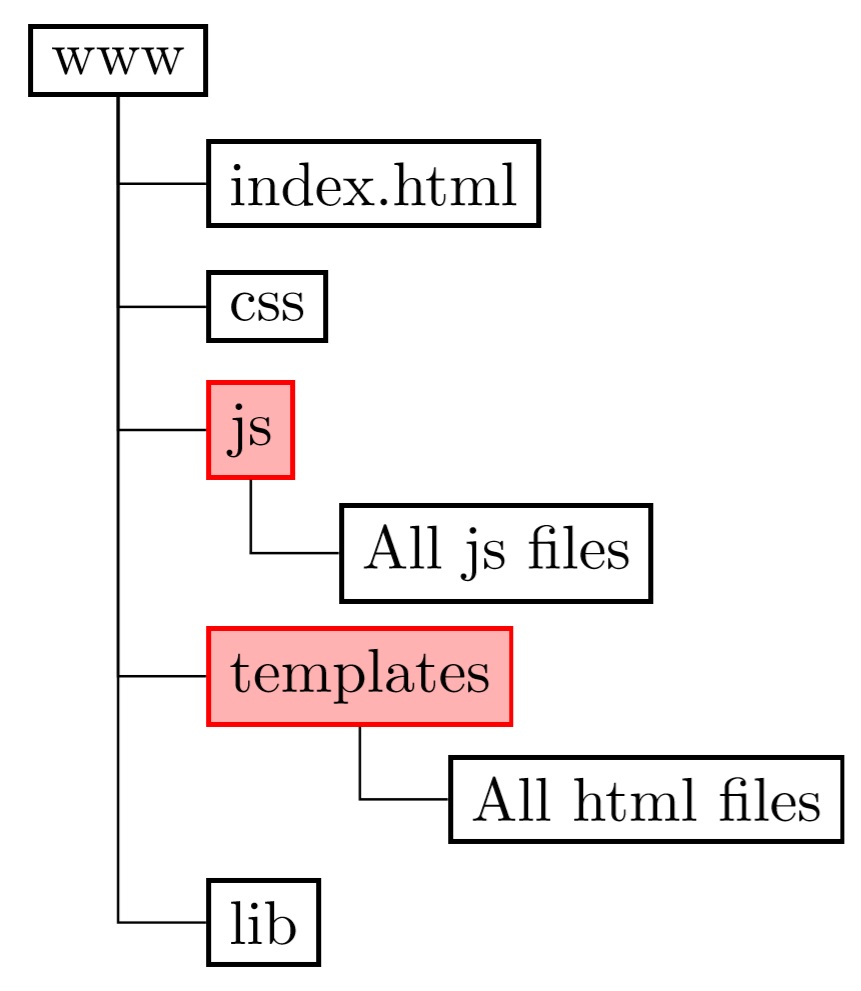
\includegraphics[width=.4\linewidth]{Images/folder_before.jpg}
  \caption{Before}
  \label{fig:before}
\end{subfigure}%
\begin{subfigure}[b]{.5\textwidth}
  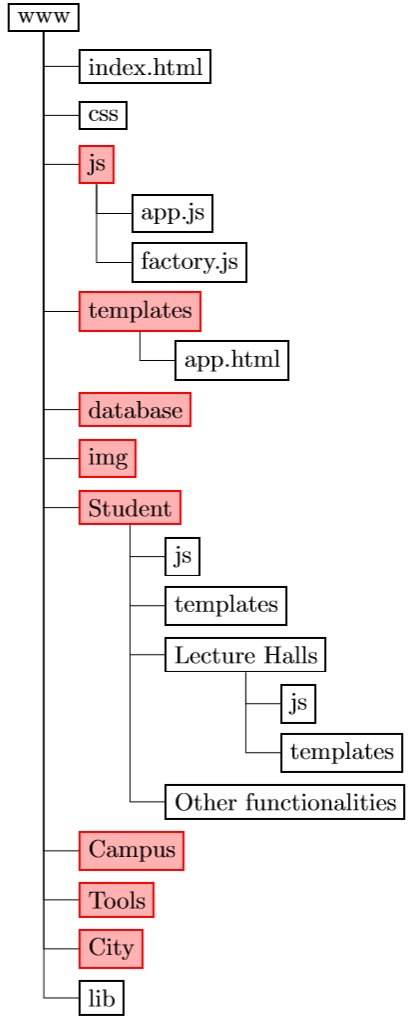
\includegraphics[width=.4\linewidth]{Images/folder_after.jpg}
  \caption{After}
  \label{fig:sub2}
\end{subfigure}
\caption{Folder evolution}
\label{fig:test}
\end{figure}

\subsection{Information processing}

Here I just explain how we treat the informations processing from an architecture's design point of view. The section 4.4 explain in detail how we did it for each specific parts.
There is a lot of external informations to relay into the application (libraries schedule, libraries addresses, daily events in the campus,...). We have two possible ways to import them.

\subsubsection{Database}

\begin{table}[H]
\begin{tabularx}{\linewidth}{>{\parskip1ex}X@{\kern4\tabcolsep}>{\parskip1ex}X}
\toprule
\hfil\bfseries Pros
&
\hfil\bfseries Cons
\\\cmidrule(r{3\tabcolsep}){1-1}\cmidrule(l{-\tabcolsep}){2-2}

Always available\par
Easy information retrieval(query)\par
Easy to modify\par
Fast\par

&

Need someone to update\par
Takes memory \par


\\\bottomrule
\end{tabularx}
\caption{Pros and cons of database}
\end{table}

\subsubsection{Web parsing}

\begin{table}[H]
\begin{tabularx}{\linewidth}{>{\parskip1ex}X@{\kern4\tabcolsep}>{\parskip1ex}X}
\toprule
\hfil\bfseries Pros
&
\hfil\bfseries Cons
\\\cmidrule(r{3\tabcolsep}){1-1}\cmidrule(l{-\tabcolsep}){2-2}

Automatic update\par
Easy information retrieval with web services(query)\par
No hardware memory consumption\par

&

Need an internet connexion and an operational server side\par
Horrible information retrieval without web services\par
If the web server change, maybe you will need to recode all the parsing method\par
Slow\par


\\\bottomrule
\end{tabularx}
\caption{Pros and cons of web parsing}
\end{table}

\iffalse
An important limitation is the need of someone in order to update database or creating new parsing system. The dream would be web services everywhere.
\fi
\subsection{Front-end and back-end}


\section{Coding standards}

\section{Security}

\section{Information retrieval}
\newpage

\chapter{The application}

In this section we will present the application as we implemented it.

\section{The application UCLCampus}

\subsection{Studies}

\subsection{Campus}

\subsection{City}

\subsection{Tools}

\subsection{Others}


\section{Modularity and how to add a new functionality}


\section{Future functionalities and possible improvements}

\chapter{Analysis}

Here we will reflect about the many choices we made and try to decide wether they were the right ones or not.

\section{Ionic framework}

\section{GitHub}

\section{Project Management}


\chapter{Conclusion} 

\chapter{Bibliography}



\end{document}